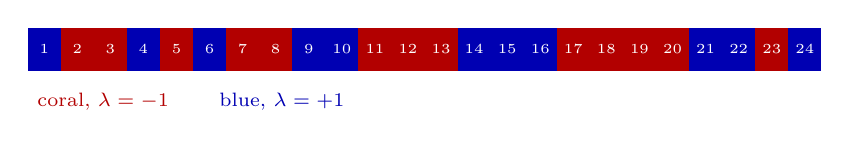
\begin{tikzpicture}[x=0.42cm,y=0.55cm]
% 1 = lambda = -1 (coral), 0 = lambda = +1 (blue). Primes are coral.
\foreach \n/\sign in {1/0,2/1,3/1,4/0,5/1,6/0,7/1,8/1,9/0,10/0,11/1,12/1,13/1,14/0,15/0,16/0,17/1,18/1,19/1,20/1,21/0,22/0,23/1,24/0}{
  \ifnum\sign=1
    \fill[red!70!black] ({\n-1},0) rectangle (\n,1);
    \node[font=\tiny,white] at ({\n-0.5},0.5) {$\n$};
  \else
    \fill[blue!70!black] ({\n-1},0) rectangle (\n,1);
    \node[font=\tiny,white] at ({\n-0.5},0.5) {$\n$};
  \fi
}
\node[font=\scriptsize,red!70!black,anchor=west] at (0,-0.7) {coral, $\lambda=-1$};
\node[font=\scriptsize,blue!70!black,anchor=west] at (5.5,-0.7) {blue, $\lambda=+1$};
\end{tikzpicture}
